\section{Funcția haotică}

Nucleul funcției hash propuse îl constituie o transformare haotică aplicată repetat asupra stării interne.
Această transformare nu se reduce la o singură funcție, ci la suprapunerea a două sisteme dinamice distincte, alese astfel încât slăbiciunile fiecăruia să fie compensate de celălalt.
Prima este baker's map, responsabilă de difuzie, iar a doua este gingerbreadman map, responsabilă de confuzie.
Compunerea lor produce, la fiecare iterație, atât amestecarea uniformă a stării, cât și o neliniaritate suficientă pentru a împiedica orice descriere algebrică simplă a procesului. \\

\subsection{Exponentul Lyapunov}

Afirmația că o funcție manifestă un comportament haotic poate fi cuantificată riguros prin intermediul exponentului Lyapunov.
Acesta măsoară rata medie cu care două traiectorii pornite din condiții inițiale infinit de apropiate se îndepărtează una de cealaltă.
Fie două puncte de start separate de o perturbație inițială $\delta_0$.
Pentru un sistem haotic, distanța dintre traiectoriile lor crește, în medie, exponențial cu numărul de iterații $n$:

\begin{equation}
    \abs{\delta_n} \approx \abs{\delta_0} \, e^{\lambda n}
\end{equation}

Coeficientul $\lambda$ din exponent este tocmai exponentul Lyapunov.
O valoare pozitivă, $\lambda > 0$, indică divergența exponențială a traiectoriilor și, implicit, sensibilitatea extremă la condițiile inițiale specifică haosului.
O valoare negativă indică, dimpotrivă, convergența traiectoriilor către o orbită stabilă. \\

\subsubsection{Liniarizarea prin matricea jacobiană}

Pentru a măsura această divergență, perturbația $\delta$ nu se urmărește prin reaplicarea funcției asupra a două puncte distincte, deoarece, după câțiva pași, distanța dintre ele depășește domeniul în care aproximarea liniară este validă.
În schimb, evoluția unei perturbații infinitezimale este descrisă de liniarizarea funcției în jurul punctului curent al traiectoriei.
Fie funcția bidimensională $F(x, y) = \left( f(x, y),\ g(x, y) \right)$.
Liniarizarea sa în punctul $p_n = (x_n, y_n)$ este dată de matricea jacobiană, care conține derivatele parțiale ale componentelor funcției:

\begin{equation}
    J(p_n) =
    \begin{pmatrix}
        \frac{\partial f}{\partial x} & \frac{\partial f}{\partial y} \\[6pt]
        \frac{\partial g}{\partial x} & \frac{\partial g}{\partial y}
    \end{pmatrix}_{p_n}
\end{equation}

Aplicată unui vector tangent $v$ (o perturbație infinitezimală), matricea jacobiană indică modul în care acel vector este rotit și scalat de o singură iterație a funcției.
Astfel, evoluția perturbației de-a lungul orbitei se reduce la o înmulțire matrice-vector la fiecare pas:

\begin{equation}
    v_{n+1} = J(p_n) \, v_n
\end{equation}

După $N$ iterații, vectorul tangent inițial $v_0$ este transformat prin produsul matricelor jacobiene evaluate succesiv în lungul traiectoriei:

\begin{equation}
    v_N = J(p_{N-1}) \, J(p_{N-2}) \cdots J(p_0) \, v_0
\end{equation}

Exponentul Lyapunov se obține ca rata medie de creștere logaritmică a normei vectorului tangent, pe măsură ce numărul de pași tinde la infinit:

\begin{equation}
    \lambda = \lim_{N \to \infty} \frac{1}{N} \ln \frac{\abs{v_N}}{\abs{v_0}}
\end{equation}

\subsubsection{Spectrul Lyapunov al unui sistem bidimensional}

Un sistem bidimensional nu posedă un singur exponent, ci un spectru de doi exponenți, $\lambda_1 \geq \lambda_2$, câte unul pentru fiecare direcție independentă a spațiului de stări.
Aceștia descriu deformarea unui disc infinitezimal de condiții inițiale: $\lambda_1$ caracterizează direcția de întindere maximă, iar $\lambda_2$ direcția de contracție.
Cel mai mare exponent, $\lambda_1$, domină comportamentul pe termen lung, fiindcă orice vector tangent ales aleatoriu se aliniază rapid direcției de creștere maximă; pozitivitatea sa este criteriul standard pentru identificarea haosului.
Suma celor doi exponenți este legată de variația ariei sub acțiunea funcției, prin logaritmul determinantului jacobian:

\begin{equation}
    \lambda_1 + \lambda_2 = \lim_{N \to \infty} \frac{1}{N} \sum_{n=0}^{N-1} \ln \abs{\det J(p_n)}
\end{equation}

Pentru o funcție care conservă aria, precum gingerbreadman map, această sumă este nulă: orice întindere pe o direcție este compensată exact de o contracție pe cealaltă.

\subsubsection{Estimarea numerică}

Calculul direct al produsului de matrice jacobiene este instabil numeric.
Deoarece toți vectorii tangenți tind să se alinieze direcției dominante, al doilea exponent devine imposibil de recuperat, iar normele cresc sau scad necontrolat, conducând la depășiri de domeniu.
Soluția standard este algoritmul lui Benettin~\cite{benettin1980}, care propagă simultan doi vectori tangenți ortonormali și îi re-ortonormalizează periodic prin procedeul Gram-Schmidt.
La fiecare pas, înainte de re-ortonormalizare, se acumulează logaritmul factorilor de creștere ai celor doi vectori; mediile acestor logaritmi, raportate la numărul de pași, converg către cei doi exponenți Lyapunov.

\begin{algorithm}[H]
    \KwData{Funcția $F$, jacobianul $J$, punctul inițial $p_0$, numărul de pași $N$}
    \KwResult{Exponenții Lyapunov $\lambda_1, \lambda_2$}
    inițializează $v_1 \gets (1, 0)$, $v_2 \gets (0, 1)$\;
    inițializează $s_1 \gets 0$, $s_2 \gets 0$\;
    \For{$n \gets 0$ \KwTo $N - 1$}{
        $v_1 \gets J(p_n) \, v_1$\;
        $v_2 \gets J(p_n) \, v_2$\;
        $r_1 \gets \abs{v_1}$;\quad $v_1 \gets v_1 / r_1$\;
        $v_2 \gets v_2 - (v_2 \cdot v_1) \, v_1$\;
        $r_2 \gets \abs{v_2}$;\quad $v_2 \gets v_2 / r_2$\;
        $s_1 \gets s_1 + \ln r_1$;\quad $s_2 \gets s_2 + \ln r_2$\;
        $p_{n+1} \gets F(p_n)$\;
    }
    $\lambda_1 \gets s_1 / N$;\quad $\lambda_2 \gets s_2 / N$\;
    \caption{Estimarea spectrului Lyapunov~\cite{benettin1980}}
\end{algorithm}

\subsection{Baker's map}

Baker's map este un sistem dinamic clasic~\cite{devaney1989}, a cărui denumire provine dintr-o analogie sugestivă cu procesul de frământare a aluatului.
Brutarul întinde aluatul pe o direcție, dublându-i lungimea, după care îl pliază la loc peste sine.
Repetarea acestui gest amestecă rapid și ireversibil orice particulă din interiorul aluatului, dispersând-o în întreaga masă.
Formal, sistemul dinamic are următoarea relație de recurență:

\begin{equation}
    (x_{n+1}, y_{n+1}) =
    \begin{cases}
        (2x_n, \frac{y_n}{2}) & \text{dacă } 0 \leq x_n < \frac{1}{2} \\
        (2 - 2x_n, 1 - \frac{y_n}{2}) & \text{dacă } \frac{1}{2} \leq x_n < 1
    \end{cases}
\end{equation}

\subsection{Gingerbreadman map}

Gingerbreadman map, introdusă de Devaney~\cite{devaney1989}, este un sistem dinamic haotic bidimensional.
Numele său provine din forma caracteristică a atractorului, care, vizualizat în plan, amintește de silueta unei figurine din turtă dulce.
Definitorie pentru această funcție este prezența valorii absolute, singura sursă de neliniaritate. \\
Formal, sistemul dinamic are următoarea relație de recurență:

\begin{equation}
    (x_{n+1}, y_{n+1}) = (1-y_n + \abs{x_n}, x_n)
\end{equation}

\subsection{Suprapunerea celor două funcții}

Cele două sisteme se completează reciproc tocmai prin slăbiciunile lor complementare.
Baker's map oferă o amestecare uniformă și lipsită de insule de stabilitate, dar este liniară.
Gingerbreadman map oferă neliniaritatea absentă din prima, dar conține regiuni cvasi-periodice.
Aplicată prima, baker's map dispersează punctul pe întregul spațiu de stări.
Astfel, dacă punctul curent se află într-o regiune cvasi-periodică a gingerbreadman map, punctul va fi împins într-o nouă orbită.
Aplicată în continuare, gingerbreadman map împletește neliniar coordonatele astfel decorelate.
În consecință, această rundă compusă, deși complet deterministă, manifestă un comportament haotic, cu o sensibilitate extremă la condițiile inițiale.
Alegerea celor două sisteme a fost motivată de faptul că ambele prezintă un comportament haotic și sunt eficiente din punct de vedere computațional.
Definițiile acestora presupun o implementare cu operații aritmetice simple, fiind utilizate tipuri de date native.

\subsection{Spectrul Lyapunov al funcțiilor}

Pentru a confirma empiric comportamentul haotic descris, spectrul Lyapunov a fost estimat numeric pentru fiecare dintre cele trei funcții, folosind algoritmul lui Benettin aplicat pe un număr mare de condiții inițiale alese aleatoriu.
Figurile următoare reprezintă cei doi exponenți, $\lambda_1$ și $\lambda_2$, codificați cromatic în funcție de valoarea lor, în planul condițiilor inițiale $(x, y)$.

\begin{figure}[!htbp]
    \centering
    \begin{minipage}{0.49\textwidth}
        \centering
        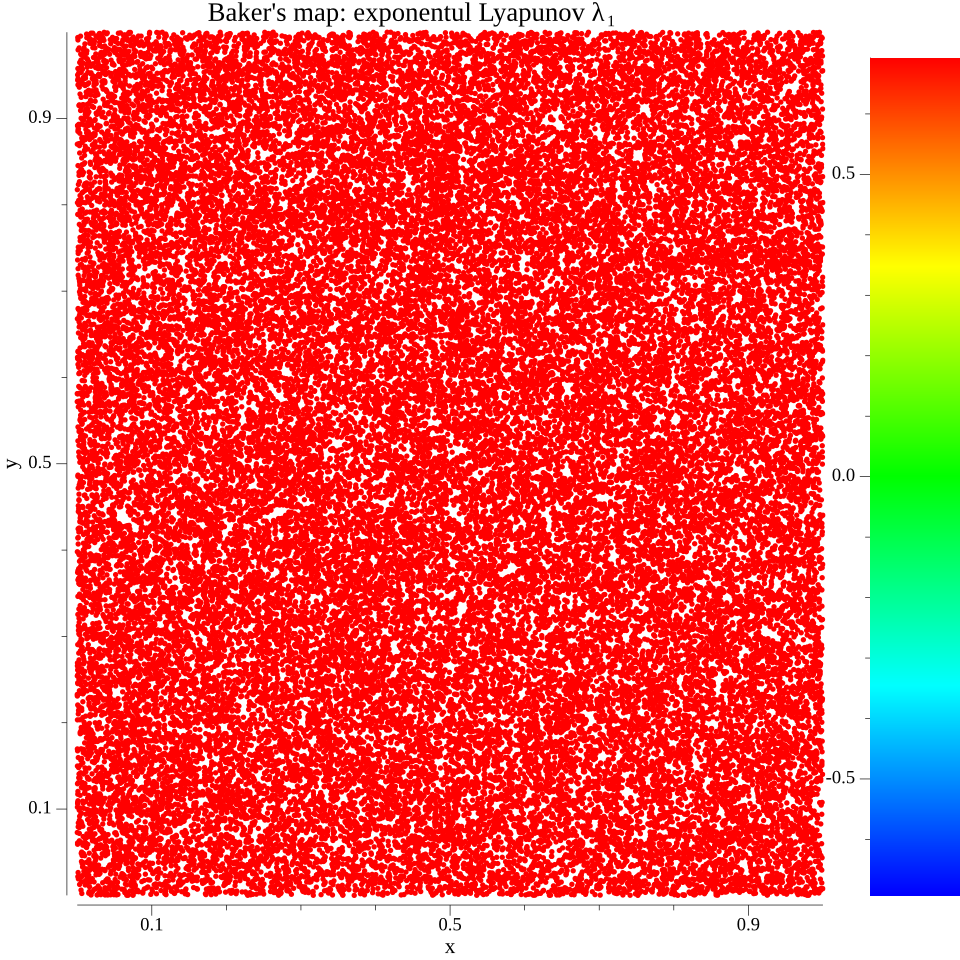
\includegraphics[width=\linewidth]{images/test-chaotic-maps-baker-lambda1.png}
    \end{minipage}
    \hfill
    \begin{minipage}{0.49\textwidth}
        \centering
        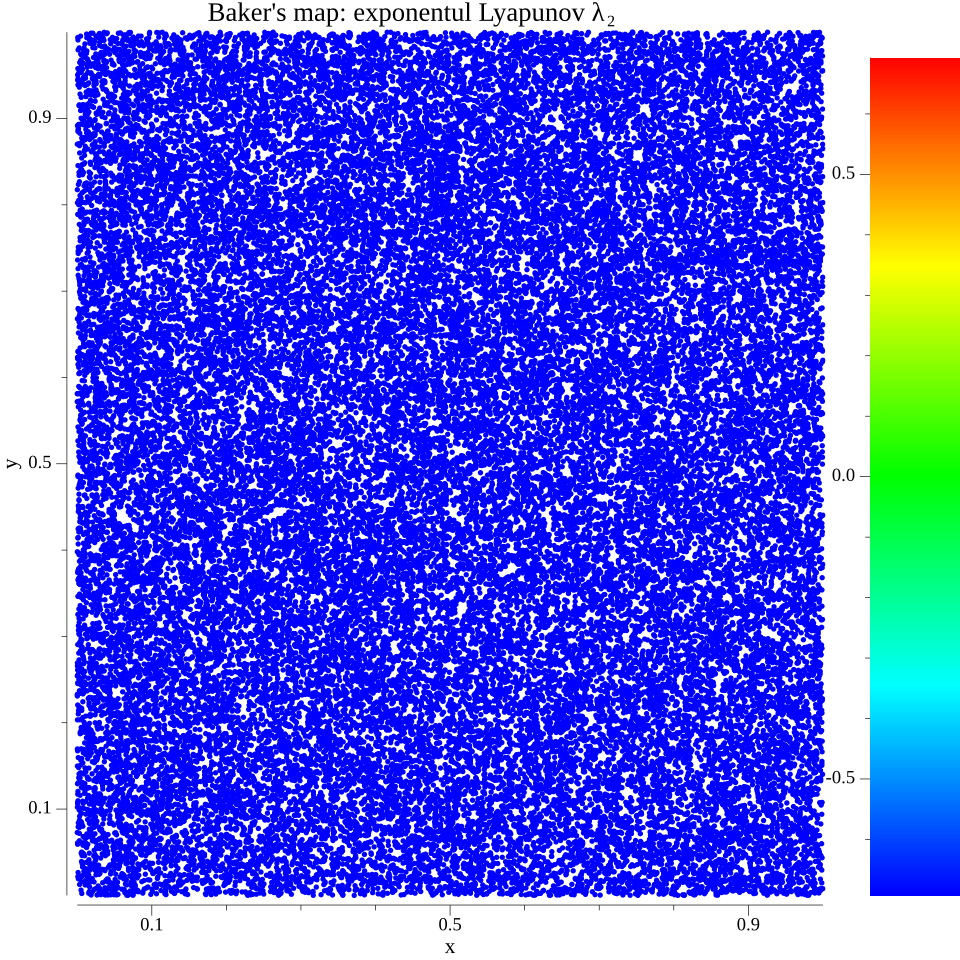
\includegraphics[width=\linewidth]{images/test-chaotic-maps-baker-lambda2.png}
    \end{minipage}
    \caption{Exponenții Lyapunov $\lambda_1$ (stânga) și $\lambda_2$ (dreapta) ai baker's map}
    \label{fig:lyapunov-baker}
\end{figure}

\begin{figure}[!htbp]
    \centering
    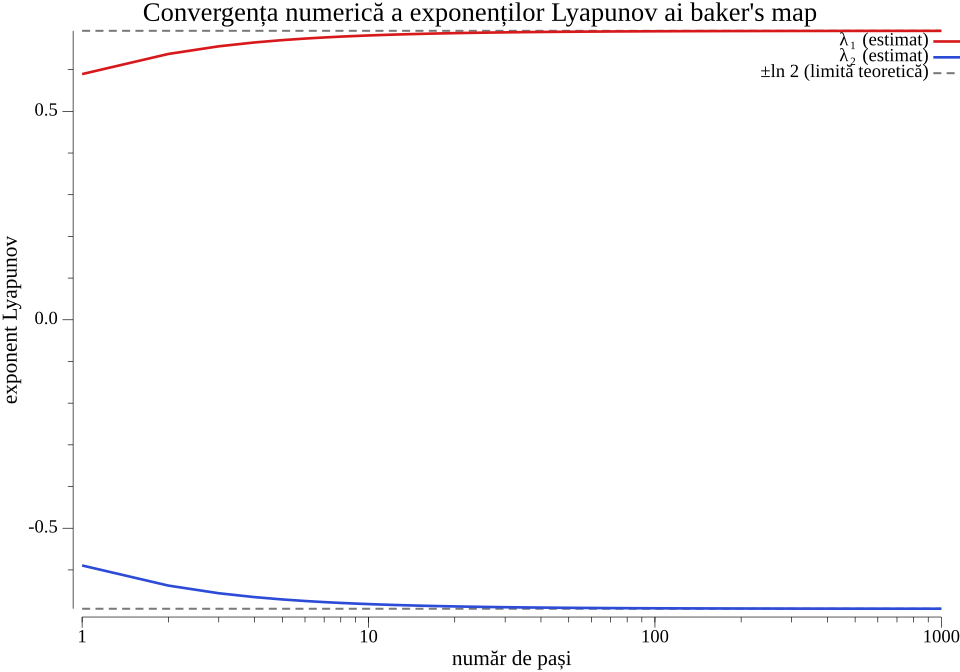
\includegraphics[width=\linewidth]{images/test-chaotic-maps-baker-convergence.png}
    \caption{Convergența numerică a exponenților Lyapunov ai baker's map către limitele teoretice $\pm\ln 2$}
    \label{fig:lyapunov-baker-convergence}
\end{figure}

\begin{figure}[!htbp]
    \centering
    \begin{minipage}{0.49\textwidth}
        \centering
        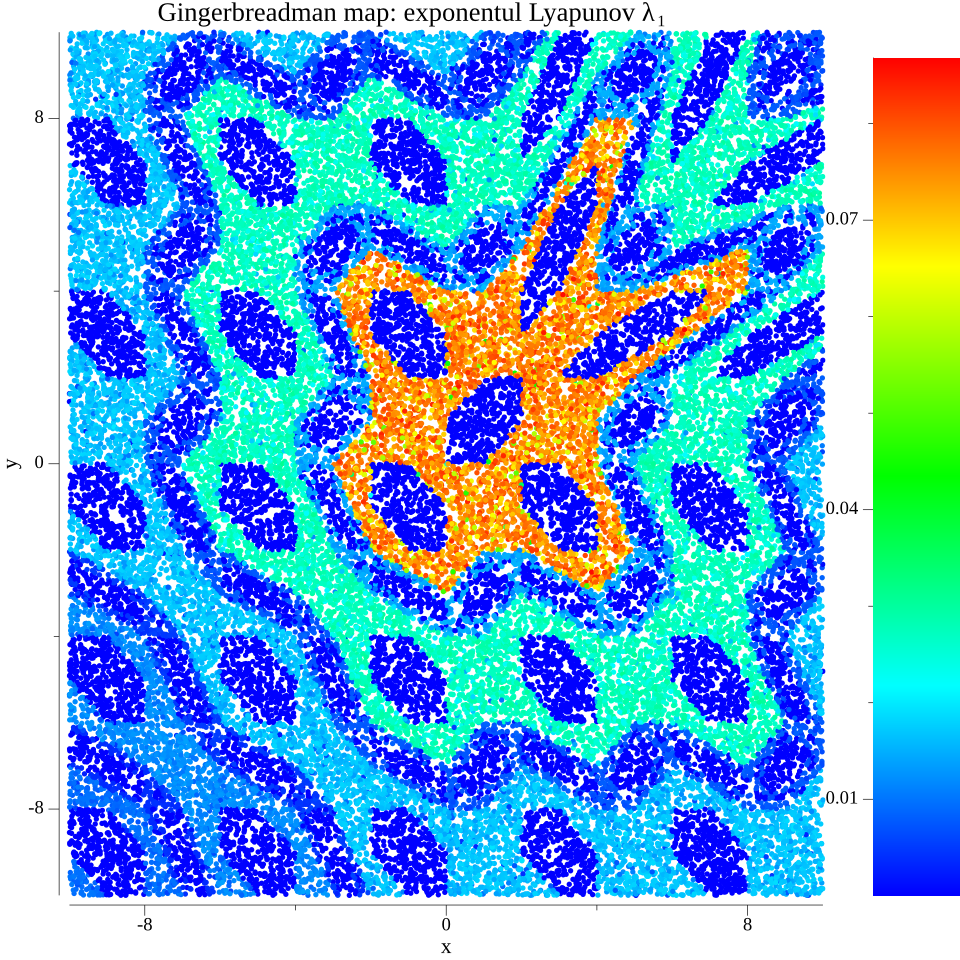
\includegraphics[width=\linewidth]{images/test-chaotic-maps-gingerbreadman-lambda1.png}
    \end{minipage}
    \hfill
    \begin{minipage}{0.49\textwidth}
        \centering
        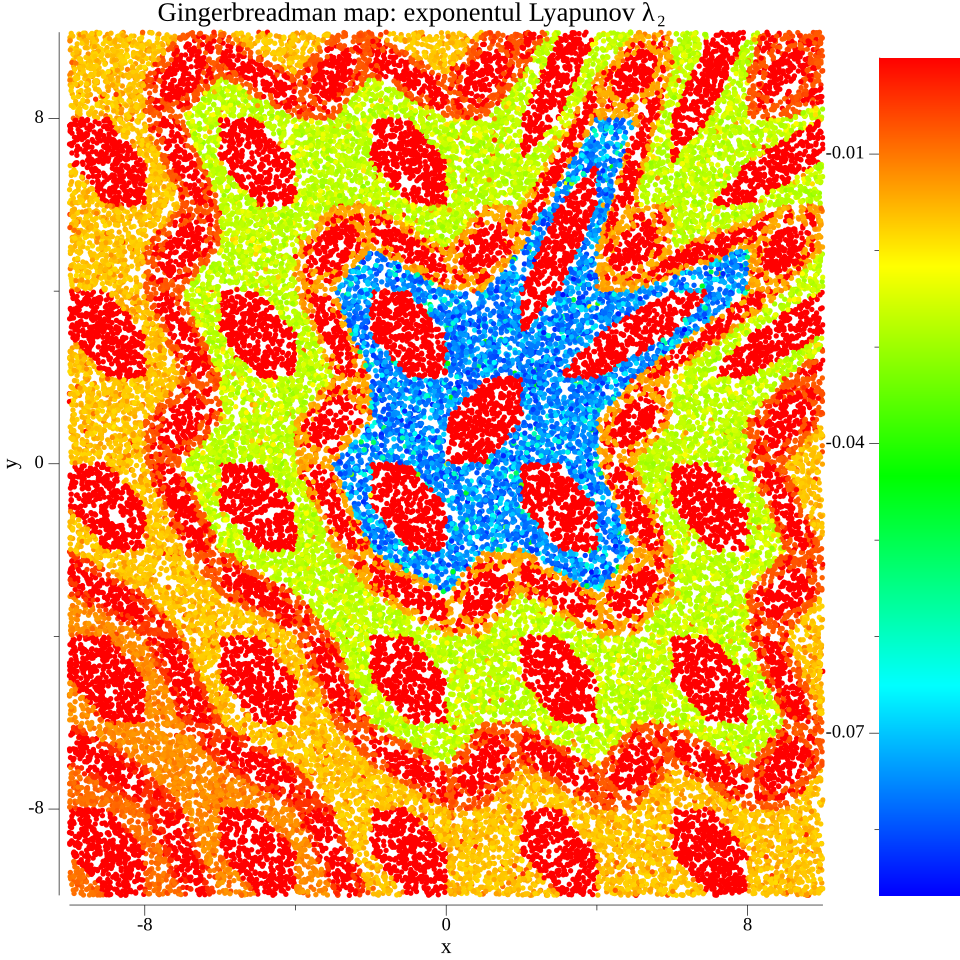
\includegraphics[width=\linewidth]{images/test-chaotic-maps-gingerbreadman-lambda2.png}
    \end{minipage}
    \caption{Exponenții Lyapunov $\lambda_1$ (stânga) și $\lambda_2$ (dreapta) ai gingerbreadman map}
    \label{fig:lyapunov-gingerbreadman}
\end{figure}

\begin{figure}[!htbp]
    \centering
    \begin{minipage}{0.49\textwidth}
        \centering
        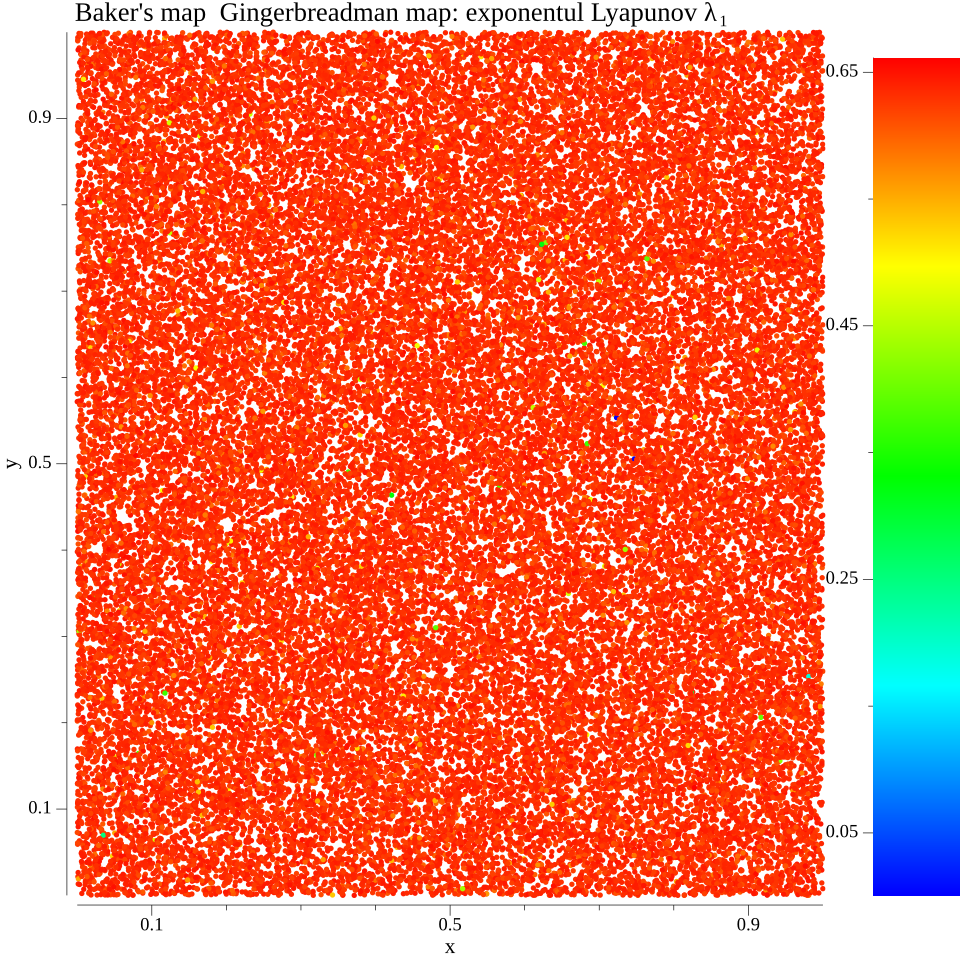
\includegraphics[width=\linewidth]{images/test-chaotic-maps-hash-lambda1.png}
    \end{minipage}
    \hfill
    \begin{minipage}{0.49\textwidth}
        \centering
        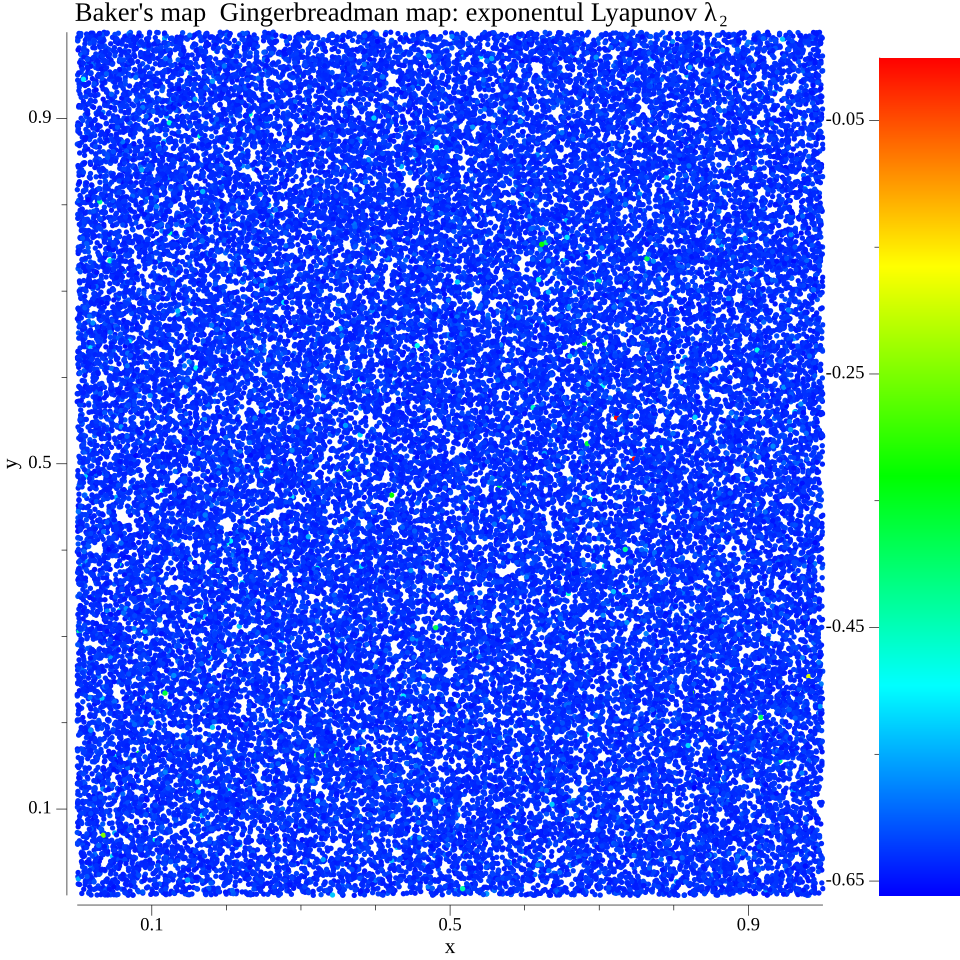
\includegraphics[width=\linewidth]{images/test-chaotic-maps-hash-lambda2.png}
    \end{minipage}
    \caption{Exponenții Lyapunov $\lambda_1$ (stânga) și $\lambda_2$ (dreapta) ai rundei compuse}
    \label{fig:lyapunov-hash}
\end{figure}

\begin{figure}[!htbp]
    \centering
    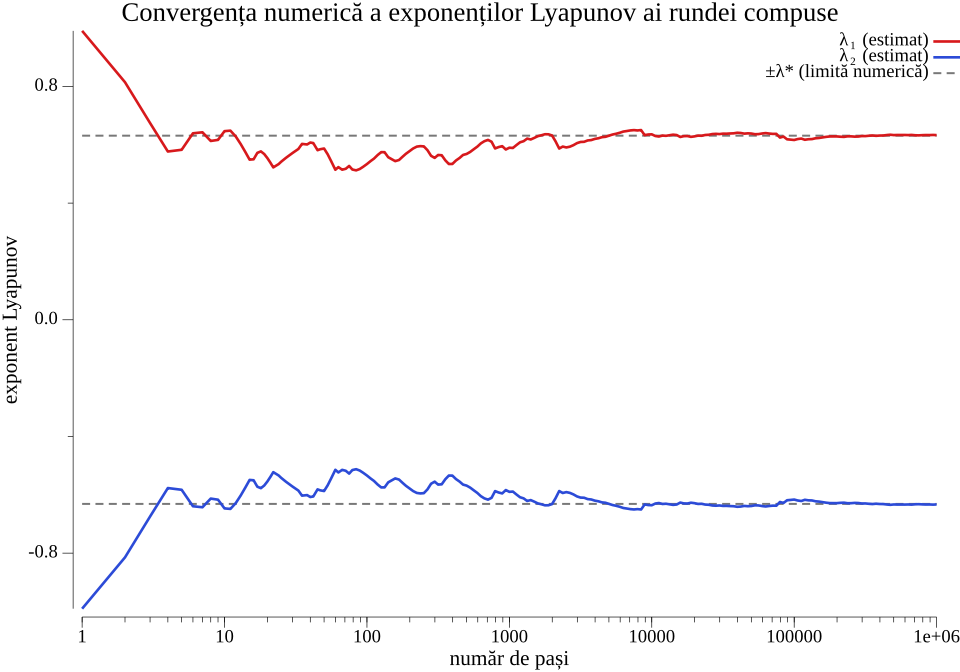
\includegraphics[width=\linewidth]{images/test-chaotic-maps-hash-convergence.png}
    \caption{Convergența numerică a exponenților Lyapunov ai rundei compuse către limita numerică $\pm\lambda^* \approx \pm0{,}6331$}
    \label{fig:lyapunov-hash-convergence}
\end{figure}

